
\documentclass[11pt]{article}
\usepackage{verbatim}
\usepackage{listings}
\usepackage{graphicx}
\usepackage{a4wide}
\usepackage{color}
\usepackage{amsmath}
\usepackage{amssymb}
\usepackage[dvips]{epsfig}
\usepackage[T1]{fontenc}
\usepackage{cite} % [2,3,4] --> [2--4]
\usepackage{shadow}
\usepackage{hyperref}
\usepackage{physics}
\usepackage{url}
\usepackage{tikz}
\usepackage{subcaption}


\usetikzlibrary{arrows, shapes}

\setcounter{tocdepth}{2}

\lstset{language=c++}
\lstset{alsolanguage=[90]Fortran}
\lstset{basicstyle=\small}
\lstset{backgroundcolor=\color{white}}
\lstset{frame=single}
\lstset{stringstyle=\ttfamily}
\lstset{keywordstyle=\color{red}\bfseries}
\lstset{commentstyle=\itshape\color{blue}}
\lstset{showspaces=false}
\lstset{showstringspaces=false}
\lstset{showtabs=false}
\lstset{breaklines}

\title{ Project 1 \\ Molecular Dynamics \\ FYS-4460 }
\author{Gullik Vetvik Killie }

\begin{document}

\maketitle

\tableofcontents

\section{Part 1:}
\subsection{Task a: Creating a FCC lattice}
	This task is implemented in the function createFCCLattice()
\\ \\
	\noindent The noble gas argon should have a stable lattice structure when a solid, by letting the system start in a stable situation we avoid a lot of energy to be infused into the systems temperature due to it minimizing potential energy. The implementation is done by going through several nodes, \(R_i\), put on a grid in the box and then placing 4 atoms around each node. Let \(c_l\) be the length between nodes.

	\begin{align*}
	\vb{R}_{ij} = \vb{R}_i + \vb{r}_j \qquad{j }= \{1,2,3,4\} \qquad{i = }\{1,2, ... , 4\text{N}_{\text{atoms}}\}
	\end{align*}

	\begin{align*}
		\vb{r}_1 &= 0 \vu{i} + 0 \vu{j} + 0 \vu{k}
		\\
		\vb{r}_2 &= \frac{c_l}{2} \vu{i} + \frac{c_l}{2} \vu{j} + 0 \vu{k}
		\\
		\vb{r}_3 &= 0 \vu{i} + \frac{c_l}{2} \vu{j} + \frac{c_l}{2} \vu{k}
		\\
		\vb{r}_4 &= \frac{c_l}{2} \vu{i} + 0 \vu{j} + \frac{c_l}{2} \vu{k}
	\end{align*}

\subsection{Task e: Computing forces}

\label{sub:potential}

		We will be using the Lennard-Jones potential to approximate the forces between the molecules, which work quite well, given it's simplicity, for neutral particles, especially noble gases, as we are dealing with in this study \cite{Wiki}. The formula is given below.

		\[
		U(r_{ij}) = 4 \epsilon \left[ \left( \frac{\sigma}{r_{ij}} \right)^{12} - \left( \frac{\sigma}{r_{ij}} \right)^{6} \right]
		\]


		
		At short distances the term to the twelfth power dominates and represents a repulsive force, Paulie exclusion principle, while at longer distances the term to sixth power dominates and represents the attractive van der Waal force. The \(\sigma \) is the distance at which the potential is \(0\), while \( \epsilon  \) is the depth of the well. 
		\(\sigma = 3.405 \text{\AA}\) and \(\varepsilon/k_B = 119.8 \text{K}\) are chosen to fit the physical properties of the system for Argon.


		\noindent The force felt between the molecules is given by the negative gradient of the potential.

		\begin{align*} 
		\vb{F}(r_{ij}) &= -\grad U(r_{ij})
		\intertext{The potential only has a nonzero derivative along \( \vb{r}_{ij} \), the  axis between then particles, so it is natural to evaluate the gradient in that coordinate system before projecting it onto the xyz coordinates used by the program.}
		\\
		\vb{F} (r_{ij}) &= - 4 \epsilon  \partial_{r_{ij}}  \left[ \left( \frac{\sigma}{r_{ij}} \right)^{12} - \left( \frac{\sigma}{r_{ij}} \right)^{6} \right] \vu{r}_{ij}
		\\
		\vb{F} (r_{ij}) &= - 4 \epsilon   \left[ -\frac{12}{r_{ij}} \left(  \frac{\sigma}{r_{ij}} \right)^{12} + \frac{6}{r_{ij}} \left( \frac{\sigma}{r_{ij}} \right)^{6} \right] \vu{r}_{ij}
		\\
		\vb{F} (r_{ij}) &= 24 \epsilon   \left[ 2 \left(  \frac{\sigma}{r_{ij}} \right)^{12} - \left( \frac{\sigma}{r_{ij}} \right)^{6} \right] \frac{\vb{r}_{ij}}{r_{ij}^2}
		\\
		m_i\pdv[2]{r_i}{t} &= \sum_j{24 \epsilon   \left[ 2 \left(  \frac{\sigma}{r_{ij}} \right)^{12} - \left( \frac{\sigma}{r_{ij}} \right)^{6} \right] \frac{\vb{r}_{ij}}{r_{ij}^2}}
		\end{align*}

	\subsection{NonDimensionality}	
	Now we introduce some new units to get a nondimensional equation of motion. 
		\(
		\begin{cases}
		r & \rightarrow   \sigma r'
		\\
		t & \rightarrow \tau t'
		\end{cases}
		\)

		\begin{align*}
		m_i\pdv[2]{\sigma r'_i}{(\tau t') }  &= \sum_j{24 \epsilon   \left[ 2 \left(  \frac{\sigma}{\sigma r'_{ij}} \right)^{12} - \left( \frac{\sigma}{\sigma r'_{ij}} \right)^{6} \right] \frac{\sigma\vb{r'}_{ij}}{\sigma^2r'^2_{ij}}}
		\\
		\pdv[2]{ r'_i}{(t')} &= \frac{24 \epsilon \tau ^2}{m_i \sigma^2}  \sum_j{  \left[ 2 \left(  \frac{\sigma}{\sigma r'_{ij}} \right)^{12} - \left( \frac{\sigma}{\sigma r'_{ij}} \right)^{6} \right] 
		\frac{\vb{r'}_{ij}}{r_{ij}'^2}}
		\intertext{Choosing \(\tau = \sigma \sqrt{ m/\varepsilon } \) then gives the dimensionless equation}
		\pdv[2]{ r'_i}{(t')} &= 24   \sum_j{  \left[ 2 r'^{-12}_{ij}  - r'^{-6}_{ij} \right] r_{ij}'^{-2}	\vb{r}'_{ij}  }
		\end{align*}



	\subsubsection{Algorithm to implement force}
		The implementation of the force will be along the following steps:
		\begin{itemize}
		\item Find vector between the two particles \( \vb{r}_{ij} = \vb{r}'_i - \vb{r}_j \)
		\item Calculate \(r_{ij}'^2\), \( r_{ij}'^6 \) and \(r_{ij}'^{12}\) for a particle pair
		\item Calculate the modified force \( 24   \sum_j{  \left[ 2 r'^{-12}_{ij}  - r'^{-6}_{ij} \right] r_{ij}'^{-2}  \vb{r}'_{ij}  } \)
		\item Add the force to both particles force account, halves the necessary computations. One positive one negative
		\end{itemize}


\appendix
	\section{Unit scheme}

	We want to use a unit system so all the numbers are computed on a unity scale, this ensures that there will be no overflow and it is easy to check that the number are approximately correct.


		The program uses a more natural set of units which let's Boltzmann's constant be 1.

		\begin{align}
			1 \text{ mass unit } &=   39.948 \text{ a.m.u } =  39.948\times 1.661\cross 10^{-27} \text{ kg}
			\\
			1 \text{ length unit } &= 3.405 \text{ \AA} = 3.405\cross 10^{-10} \text{ m}
			\\
			1 \text{ energy unit } &= 1.651 \cross 10^{-21} \text{ J}
			\\
			1 \text{ temperature unit } &= 119.735 \text{ K}
		\end{align}


	All the other units are then expressed in term of these units.

	Boltzmann constant translates between temperature and energy, in SI-units it is \( k_B = 1.381 \cross 10^{-23} \text{ J K}^{-1}\), which in the previously defined units becomes
	\begin{align}
	k_B &= 1.381 \cross 10^{-23}  \left(\text{ J K}^{-1}\right)  \left(\frac{\text{energy unit}}{1.651 \cross 10^{-21} \text{ J}}\right)
	\left( \frac{119.735 \text{ K}}{\text{temperature unit}} \right)
	\\
	k_B &= 1 \; \frac{\text{energy unit}}{\text{temperature unit}}
	\end{align}

































% \subsection{Task a: Periodic boundary conditions}
% 	This task was implemented in the function applyPeriodicBoundaryConditions() and the program can be found at the github page \cite{myGit}.
% \\ \\
% 	\noindent Since we have limited computational power we are only working on a small piece of argon material, to get away from boundary cases we simulate a system of infinite size by implementing periodic boundary conditions. This is done by confining the atoms in a box and each time a particle reaches the end of the box it is put to the other side.

% \subsection{Task b: Removing momentum}
% 	This task is implemented in the function removeMomentum().
% \\ \\
% 	\noindent Since all the atoms are given random velocities the net momentum is not zero and the cloud will drift. This is solved by calculating the total momentum of all the atoms, and then subtracting a fraction of the total momentum from each atom so the total momentum ends up being zero.

% \subsection{Task c: Putting the atoms on a lattice}
% 	This task is implemented in the function createFCCLattice()
% \\ \\
% 	\noindent The noble gas argon should have a stable lattice structure when a solid, by letting the system start in a stable situation we avoid a lot of energy to be infused into the systems temperature due to it minimizing potential energy. The implementation is done by going through several nodes, \(R_i\), put on a grid in the box and then placing 4 atoms around each node. Let \(c_l\) be the length between nodes.

% 	\begin{align*}
% 	\vb{R}_{ij} = \vb{R}_i + \vb{r}_j \qquad{j }= \{1,2,3,4\} \qquad{i = }\{1,2, ... , 4\text{N}_{\text{atoms}}\}
% 	\end{align*}

% 	\begin{align*}
% 		\vb{r}_1 &= 0 \vu{i} + 0 \vu{j} + 0 \vu{k}
% 		\\
% 		\vb{r}_2 &= \frac{c_l}{2} \vu{i} + \frac{c_l}{2} \vu{j} + 0 \vu{k}
% 		\\
% 		\vb{r}_3 &= 0 \vu{i} + \frac{c_l}{2} \vu{j} + \frac{c_l}{2} \vu{k}
% 		\\
% 		\vb{r}_4 &= \frac{c_l}{2} \vu{i} + 0 \vu{j} + \frac{c_l}{2} \vu{k}
% 	\end{align*}


% \subsection{Task d: Implementing a Verlet integrator}


% 	\label{sub:verlet}
% 		The Integrator is a widely used integrator in  molecular dynamics \cite{compPhys} because of it's properties as a symplectic integrator which means that it conserves areas in phase space very well and it allows stable integration of the equation of motion \cite{aBInitio}. Newton's second law for for a particle in our molecule ensemble reads:

% 		\[m\pdv[2]{x_{i}}{t} = F_{i}\]

% 		\[\pdv{x_{i}}{t} = v_{i} \text{     and     } \pdv{v_{i}}{t} = \frac{F_{i}}{m} \]

% 		The Leapfrog algorithm is a slight continuation on the Verlet algorithm doing the step in two steps. Doing a Taylor expansion around both the step and half the step we get.
	

% 		\begin{align}
% 			x_{i}(t+h) &= x_i(t) + hx_i'(t) + \frac{h^2}{2}x_i''(t) + \order{h^3} \label{eq:leapfrog_start}
% 			\\
% 			x_i'(t+ \frac{h}{2} ) &= x_i'(t) + \frac{h}{2} x_i''(t) + \order{h^2} \label{eq:leapfrog_half}
% 		\end{align}	

% 		\noindent Inserting equation \eqref{eq:leapfrog_half} into \eqref{eq:leapfrog_start} to obtain

% 		\begin{equation}
% 		x_{i}(t+h) = x_i(t) + hx_i'(t+ \frac{h}{2})+ \order{h^3} \label{eq:leapfrog_pos_step}
% 		\end{equation}

% 		\noindent A Taylor first order expansion of the velocity produces the following

% 		\begin{align}
% 			x'_i(t+\frac{h}{2}) &= x_i'(t)  + \frac{h}{2}x_i''(t) + \order{h^2} \label{eq:leapfrog_vel_step}
% 		\end{align}

% 		\noindent By using equation \eqref{eq:leapfrog_vel_step}, then \eqref{eq:leapfrog_pos_step} and then \eqref{eq:leapfrog_vel_step} again we obtain \(x_i(t+h)\) and \(v_i(t+h)\). The algorithm follows:

% 		\begin{align*}
% 		v_i(t+\frac{h}{2}) &= x_i'(t)  + \frac{h}{2}\frac{F_i(t)}{m} + \order{h^2} 
% 		\\
% 		x_i(t+h) &= x_i(t) + hx_i'(t+ \frac{h} {2} ) + \order{h ^ 3}
% 		\\
% 		v_i(t+h) &= v_i(t+\frac{h}{2})  +  \frac{h}{2}\frac{F_i(t+ \frac{h}{2})}{m} + \order{h^2} 
% 		\end{align*}

% \subsection{Task e: Computing forces}

% \label{sub:potential}
% 		We will be using the Lennard-Jones potential to approximate the forces between the molecules, which work quite well, given it's simplicity, for neutral particles, especially noble gases, as we are dealing with in this study \cite{Wiki}. The formula is given below.

% 		\[
% 		U(r_{ij}) = 4 \epsilon \left[ \left( \frac{\sigma}{r_{ij}} \right)^{12} - \left( \frac{\sigma}{r_{ij}} \right)^{6} \right]
% 		\]
		
% 		At short distances the term to the twelfth power dominates and represents a repulsive force, Paulie exclusion principle, while at longer distances the term to sixth power dominates and represents the attractive van der Waal force. The \(\sigma \) is the distance at which the potential is \(0\), while \( \epsilon  \) is the depth of the well. \\
% 		Experimentally the following values for argon has been found: 
% 		\(
% 		\begin{cases}
% 		\epsilon/k_B &= 119.8 \text{K} 
% 		\\
% 		\sigma &= 3.405 \text{\AA}
% 		\end{cases}
% 		\)


% 		\noindent The force felt between the molecules is given by the negative gradient of the potential.

% 		\begin{align*} 
% 		\vb{F}(r_{ij}) &= -\grad U(r_{ij})
% 		\intertext{The potential only has a nonzero derivative along \( \vb{r}_{ij} \), the  axis between then particles, so it is natural to evaluate the gradient in that coordinate system before projecting it onto the xyz coordinates used by the program.}
% 		\\
% 		\vb{F} (r_{ij}) &= - 4 \epsilon \vu{r}_{ij} \partial_{r_{ij}}  \left[ \left( \frac{\sigma}{r_{ij}} \right)^{12} - \left( \frac{\sigma}{r_{ij}} \right)^{6} \right]
% 		\\
% 		\vb{F} (r_{ij}) &=- 4 \epsilon \vu{r}_{ij} \left[ \left( -\frac{12}{\sigma} \right) \left( \frac{\sigma}{r_{ij}}  \right)^{13} 
% 		- \left( - \frac{6}{\sigma}  \right)\left( \frac{\sigma}{r_{ij}} \right)^{7} \right]
% 		\intertext{Then it is projected onto the xyz coordinates, 
% 		\( F_k = \left(F\frac{r_{ij}}{\abs{r_{ij}}}\right)_k= F\frac{k_{ij}}{\abs{r_{ij}}} \), where \( k_{ij} \) is the distance between the particles in direction \(k = \{x,y,z\}\) , and \( \abs{r_{ij}} \) is the total distance.
% 		}
% 		F_k &=  \frac{24}{\sigma} \epsilon \left[ 2  \left( \frac{\sigma}{r_{ij}}  \right)^{13} 
% 		- \left( \frac{\sigma}{r_{ij}} \right)^{7} \right]\frac{k_{ij}}{\abs{r_{ij}}}
% 		\end{align*}

% 	\subsubsection{Algorithm to implement force}
% 		The implementation of the force will be along the following steps:
% 		\begin{itemize}
% 		\item Calculate \(r_{ij} = \abs{\vb{r}_i - \vb{r}_j}\) for a particle pair
% 		\item Calculate \(F_{r_{ij}} =  \frac{24}{\sigma} \epsilon \left[ 2  \left( \frac{\sigma}{r_{ij}}  \right)^{13} 
% 		- \left( \frac{\sigma}{r_{ij}} \right)^{7} \right]\)
% 		\item Calculate \(F_x = F_{r_{ij}} \frac{k_{ij}}{\abs{r_{ij}}} \) for xyz
% 		\item Add the force to both particles force account, halves the necessary computations. One positive one negative
% 		\end{itemize}


% \subsection{Task f: Calculating some statistical properties}
% 	\subsubsection{Kinetic energy}

% 		The kinetic energy is found trough adding up the kinetic energy for all the atoms separately. It is straight forward and done in a function, in the statisticsSampler class, called sampleKineticEnergy(). It goes through all the atoms and adds it's contribution to the total kinetic energy. 

% 		\[
% 		E_k = \sum\limits^{N_{atoms}}_{i=1}{\frac{1}{2}m_i v_i^2}
% 		\]

% 		\noindent Then it also stores the instantaneous temperature of the substance which is given by the equipartition theorem \( \langle E_K \rangle = \frac{2}{3} k_B N_{atoms} T \). By looking at the kinetic energy in a time-instant instead of averaging it we get an instantaneous temperature.
% \\ \\
% 		\noindent All of this is stored together with the potential energy to a text file "./statisticalResults/statisticalValues.tsv" which can be plotted by the python program plots.py.

% \subsection{Task g: implementing Neighbor cells}
% 	A simple system of \(3\cross 3\) neighbors, see figure \ref{fig:neighbor_grid} will have all the properties and connections of a larger system, since a neighbor is only connected to the neighbors bordering it. Let us choose the neighbor in the center, \(111\),  and find the neighbors we must go through to find to let it interact with each of it's neighbors once. First we let it interact with the top layer, \ref{fig:top}, and then we note that it is not necessary to let it interact with the bottom layer, since all the cells in that layer will interact with the choosen cell, \(111\). Then we fill the remainer of the front, 

% 	\tikzstyle{vertex}=[circle,fill=black!25,minimum size=20pt,inner sep=0pt]

% 	\begin{figure}
% 		\begin{subfigure}{1\textwidth}
% 			\begin{subfigure}[b]{0.18\textwidth}
% 			\begin{tikzpicture}[scale=1.0, auto,swap]
% 	    		\foreach \pos/\name in {{(2,0)/200}, 	{(2,1)/201},	{(2,2)/202},
% 	                            		{(1,0)/000}, 	{(1,1)/101}, 	{(1,2)/102},
% 	                            		{(0,0)/000}, 	{(0,1)/001},	{(0,2)/002}}
% 	        	\node[vertex] (\name) at \pos {$\name$};
% 	        \end{tikzpicture}
% 	        \caption*{j \(= 0\)}
% 	        \end{subfigure}
% 	        \qquad \qquad
% 	        \begin{subfigure}[b]{0.18\textwidth}
% 			\begin{tikzpicture}[scale=1.0, auto,swap]
% 	    		\foreach \pos/\name in {{(2,0)/210}, 	{(2,1)/211},	{(2,2)/212},
% 	                            		{(1,0)/010}, 	{(1,1)/111}, 	{(1,2)/112},
% 	                            		{(0,0)/010}, 	{(0,1)/011},	{(0,2)/012}}
% 	        	\node[vertex] (\name) at \pos {$\name$};
% 	        \end{tikzpicture}
% 	        \caption*{j \(= 1\)}
% 	        \end{subfigure}
% 	        \qquad \qquad
% 	        \begin{subfigure}[b]{0.18\textwidth}
% 			\begin{tikzpicture}[scale=1.0, auto,swap]
% 	    		\foreach \pos/\name in {{(2,0)/220}, 	{(2,1)/221},	{(2,2)/222},
% 	                            		{(1,0)/020}, 	{(1,1)/121}, 	{(1,2)/122},
% 	                            		{(0,0)/020}, 	{(0,1)/021},	{(0,2)/022}}
% 	        	\node[vertex] (\name) at \pos {$\name$};
% 	        \end{tikzpicture}
% 	        \caption*{j \(= 2\)}
% 	        \end{subfigure}
% 	       	\caption{All the neighbors in a \(3\cross 3\) system divided up into three slices with j constant. The numbers are position in an ijk-grid.}
% 	       	\label{fig:neighbor_grid}
% 		\end{subfigure}
% 		\begin{subfigure}{1\textwidth}
% 			\begin{subfigure}[b]{0.18\textwidth}
% 			\begin{tikzpicture}[scale=1.0, auto,swap]
% 	    		\foreach \pos/\name in {{(0,2)/X}, 	{(1,2)/X},	{(2,2)/X},
% 	                            		{(0,1)/}, 	{(1,1)/}, 	{(2,1)/},
% 	                            		{(0,0)/*}, 	{(1,0)/*},	{(2,0)/*}}
% 	        	\node[vertex] (\name) at \pos {$\name$};
% 	        \end{tikzpicture}
% 	        \caption*{j \(= 0\)}
% 	        \end{subfigure}
% 	        \qquad \qquad
% 	        \begin{subfigure}[b]{0.18\textwidth}
% 			\begin{tikzpicture}[scale=1.0, auto,swap]
% 	    		\foreach \pos/\name in {{(0,2)/X}, 	{(1,2)/X},	{(2,2)/X},
% 	                            		{(0,1)/}, 	{(1,1)/O}, 	{(2,1)/},
% 	                            		{(0,0)/*}, 	{(1,0)/*},	{(2,0)/*}}
% 	        	\node[vertex] (\name) at \pos {$\name$};
% 	        \end{tikzpicture}
% 	        \caption*{j \(= 1\)}
% 	        \end{subfigure}
% 	        \qquad \qquad
% 	        \begin{subfigure}[b]{0.18\textwidth}
% 			\begin{tikzpicture}[scale=1.0, auto,swap]
% 	    		\foreach \pos/\name in {{(0,2)/X}, 	{(1,2)/X},	{(2,2)/X},
% 	                            		{(0,1)/}, 	{(1,1)/}, 	{(2,1)/},
% 	                            		{(0,0)/*}, 	{(1,0)/*},	{(2,0)/*}}
% 	        	\node[vertex] (\name) at \pos {$\name$};
% 	        \end{tikzpicture}
% 	        \caption*{j \(= 2\)}
% 	        \end{subfigure}
% 	       	\caption{Let the center cell interact with the top layer. 'X' represents a cell that the center cell, 'O' has interacted with. '*' represents a cell that will interact with the center cel, 'O' if it undergoes the same scheme as the center cell 'O'.}
% 	       	\label{fig:top}
% 		\end{subfigure}
% 		\begin{subfigure}{1\textwidth}
% 			\begin{subfigure}[b]{0.18\textwidth}
% 			\begin{tikzpicture}[scale=1.0, auto,swap]
% 	    		\foreach \pos/\name in {{(0,2)/X}, 	{(1,2)/X},	{(2,2)/X},
% 	                            		{(0,1)/*}, 	{(1,1)/}, 	{(2,1)/X},
% 	                            		{(0,0)/*}, 	{(1,0)/*},	{(2,0)/*}}
% 	        	\node[vertex] (\name) at \pos {$\name$};
% 	        \end{tikzpicture}
% 	        \caption*{j \(= 0\)}
% 	        \end{subfigure}
% 	        \qquad \qquad
% 	        \begin{subfigure}[b]{0.18\textwidth}
% 			\begin{tikzpicture}[scale=1.0, auto,swap]
% 	    		\foreach \pos/\name in {{(0,2)/X}, 	{(1,2)/X},	{(2,2)/X},
% 	                            		{(0,1)/*}, 	{(1,1)/O}, 	{(2,1)/X},
% 	                            		{(0,0)/*}, 	{(1,0)/*},	{(2,0)/*}}
% 	        	\node[vertex] (\name) at \pos {$\name$};
% 	        \end{tikzpicture}
% 	        \caption*{j \(= 1\)}
% 	        \end{subfigure}
% 	        \qquad \qquad
% 	        \begin{subfigure}[b]{0.18\textwidth}
% 			\begin{tikzpicture}[scale=1.0, auto,swap]
% 	    		\foreach \pos/\name in {{(0,2)/X}, 	{(1,2)/X},	{(2,2)/X},
% 	                            		{(0,1)/*}, 	{(1,1)/}, 	{(2,1)/X},
% 	                            		{(0,0)/*}, 	{(1,0)/*},	{(2,0)/*}}
% 	        	\node[vertex] (\name) at \pos {$\name$};
% 	        \end{tikzpicture}
% 	        \caption*{j \(= 2\)}
% 	        \end{subfigure}
% 	       	\caption{Then we let the center cell interact with the rest of the front, i-direction.}
% 	       	\label{fig:front}
% 		\end{subfigure}
% 		\begin{subfigure}{1\textwidth}
% 			\begin{subfigure}[b]{0.18\textwidth}
% 			\begin{tikzpicture}[scale=1.0, auto,swap]
% 	    		\foreach \pos/\name in {{(0,2)/X}, 	{(1,2)/X},	{(2,2)/X},
% 	                            		{(0,1)/*}, 	{(1,1)/X}, 	{(2,1)/X},
% 	                            		{(0,0)/*}, 	{(1,0)/*},	{(2,0)/*}}
% 	        	\node[vertex] (\name) at \pos {$\name$};
% 	        \end{tikzpicture}
% 	        \caption*{j \(= 0\)}
% 	        \end{subfigure}
% 	        \qquad \qquad
% 	        \begin{subfigure}[b]{0.18\textwidth}
% 			\begin{tikzpicture}[scale=1.0, auto,swap]
% 	    		\foreach \pos/\name in {{(0,2)/X}, 	{(1,2)/X},	{(2,2)/X},
% 	                            		{(0,1)/*}, 	{(1,1)/O}, 	{(2,1)/X},
% 	                            		{(0,0)/*}, 	{(1,0)/*},	{(2,0)/*}}
% 	        	\node[vertex] (\name) at \pos {$\name$};
% 	        \end{tikzpicture}
% 	        \caption*{j \(= 1\)}
% 	        \end{subfigure}
% 	        \qquad \qquad
% 	        \begin{subfigure}[b]{0.18\textwidth}
% 			\begin{tikzpicture}[scale=1.0, auto,swap]
% 	    		\foreach \pos/\name in {{(0,2)/X}, 	{(1,2)/X},	{(2,2)/X},
% 	                            		{(0,1)/*}, 	{(1,1)/*}, 	{(2,1)/X},
% 	                            		{(0,0)/*}, 	{(1,0)/*},	{(2,0)/*}}
% 	        	\node[vertex] (\name) at \pos {$\name$};
% 	        \end{tikzpicture}
% 	        \caption*{j \(= 2\)}
% 	        \end{subfigure}
% 	       	\caption{Then we let the center cell interact with side, j-direction and all the neighboring cells to cell \(111\) is interacted with, or interacts with cell \(111\) when all the cells are run trough.}
% 	       	\label{fig:side}
% 		\end{subfigure}
% 		\caption{A schematic explanation of the algorithm to go through all the neighboring cells of a neighbor cell.}
% 	\end{figure}
		




% 	\begin{table}
% 		\begin{tabular}{| c | c | c | c | c | c | c | c | c |}
% 		\hline
% 			\(N_{atoms}\)	&	4 			&	32			&	108			&	256		&	500		&	864		& 1372		&	2048
% 			\\ \hline
% 			time (s)		&	0.003539	&	0.054251	&	0.274064	&	1.22426	&	3.96325	&	11.3712	& 28.3554	& 62.9434 
% 			\\ \hline
% 			time (s) with list & -			& 0.179424		&	1.74696		&	2.89621	&	9.14402	&	13.3765	& 33.5662	& 39.6798
% 			\\ \hline
% 		\end{tabular}
% 		\caption{This table shows time to compute 100 timesteps with different amount of atoms in the model. The time is increasing much faster than linearly. After the neighborlists are implemented it is slower on very few atoms, but it grows slower and spends less time aabove 2048 atoms.}
% 	\label{tab:time_spent}
% 	\end{table}

% 	Table \ref{tab:time_spent} shows the time spent computing with different amount of atoms in the system, as the system increases the time is increasing fast and we can see the need to implement neighbor cells. The time is increasing fast because the program has to calculate the forces between all the atoms and that is of the order \(\order{N^2}\). By only calculating the nearby atoms, which will be the ones affecting each other the most, the time taken will mostly increase linearly.
% \\ \\
% 	\noindent The force is mostly ignorable outside a distance of \(3 \sigma \), see figure \ref{fig:force}.

% 	\begin{itemize}
% 		\item Divide box into smaller boxes with \(l >3\sigma\), and put the cell layer class between the system and atoms.
% 				\[\text{system} \rightarrow\text{cellbox} \rightarrow \text{atoms}\]
% 		\item For each box go through all the boxes neighboring boxes. Boxes should be stored in three lists as \((i,j,k)\) and the neighboring boxes to box \((i,j,k)\) are \( (i-1, j-1, k-1), (i-1,j-1,k) \) and going through all the combinations to \( (i+1,j+1,k+1) \)
% 		\item Each atom needs an additional box assignment property
% 		\item Calculate the forces for all the atoms belonging to the neighboring boxes
% 	\end{itemize}

	
% 	\begin{figure}
% 		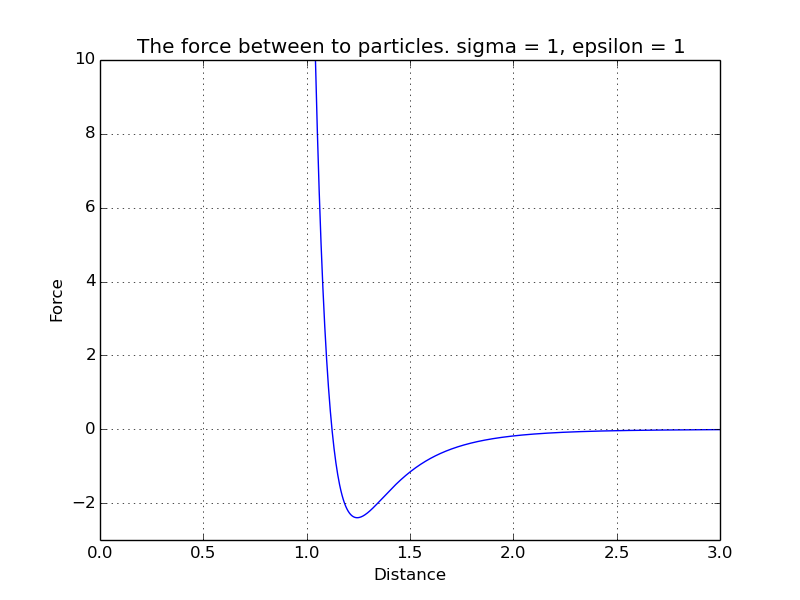
\includegraphics[scale = 0.5]{Figures/forcePlot}
% 		\caption{A picture over the force felt between two particles due to the Lennard-Jones potential. At approximately 3 \(\sigma\) of length the magnitude of the force closes to zero and we can ignore the contribution of atoms further away from each other.}
% 		\label{fig:force}
% 	\end{figure}

% \subsection{Task g: Implementing a thermostat}
% 	After initializing the system, it will after while stabilize with a different temperature than it was initialized in. So we will need to implement a thermostat and let that run for a while to get the system to maintain that temperature that we want to measure statistical properties at. In this project we will implement a Berendsen thermostat, that works by first calculating a scalar value ,\(\gamma\), for how much the temperature of the system is different from the wanted temperature, see equation \eqref{eq:berentsen}, where \(\gamma\) is the adjustment scalar, \( \Delta t \) is the timestep, \( T_Bath \text{ and } T\) is the measured and wanted temperatures, \(\tau\) is a relaxation factor. 

% 	\begin{align}
% 		\gamma &= \sqrt{ 1 - \frac{\Delta t}{\tau} \left( \frac{T_{Bath}}{T} - 1 \right) } \label{eq:berentsen}
% 	\end{align}

% 	Then all of the individual atoms velocities are multiplied with the factor \( \gamma\) and the temperature is increased, or decreases, to get closer to the wanted temperature.

% \section{Part 2: Saving and loading in binary format}
% \subsection{Task a:}
% 	The save and load functions, in binary, was implemented as members in the system class and are called load() and save. They load all the positions and velocities of all the particles in the system.

% \subsection{Task b: Writing the statistical properties to file }
% 	In the class statisticsSampler there all the statistical properties are sampled and written to a file. They are stored as "./statisticalResults/statisticalValues.csv"


% \subsection{Task c: Measure the pressure}
	
% 	The pressure for a molecular system can be calculated with the following equation, \eqref{eq:press} (for an NVT ensemble, it also works quite well for an NVE ensemble), where $\rho_n$ is the number density, $k_B$ is the Boltzmann constant, $T$ is the temperature, $V$ is the volume, $\vec r_i$ is the position of atom $i$ and $\vec F_i$ is the total force on atom $i$:

% 	\begin{align}
%     P &= \rho_n k_B T + \frac{1}{3V}\Bigg \langle \sum_{i=1}^N \vb F_i \cdot \vb r_i \Bigg\rangle \label{eq:press}
%     \intertext{The force on one atom is the sum of all the force felt from all the other atoms \( \vb{F}_i = \sum_{j=1, i \ne j}^N \vb F_{ij } \)}
%     P &= \rho_n k_B T + \frac{1}{3V}\Bigg \langle \sum_{i=1}^N \left( \sum_{j=1, i \ne j}^N \vb F_{ij}  \right)\cdot \vb r_i \Bigg\rangle
%     \intertext{The \(\vb r_{i} \) can be moved into the \(j-\)summation since it is not dependent on \(j\)}
%     P &= \rho_n k_B T + \frac{1}{3V}\Bigg \langle \sum_{i=1}^N \left( \sum_{j=1, j \ne i}^N \vb F_{ij}  \cdot \vb r_i  \right) \Bigg\rangle
% 	\end{align}


% 	\begin{align}
%     P = \rho_n k_B T + \frac{1}{3V}\Bigg\langle \sum_{i>j} \vec r_{ij} \cdot \vec F_{ij} \Bigg\rangle,
% 	\end{align}

% \subsection{Task d:}
% 	Here we will start up a new system of \(4000\) atoms with an initial temperature of \(300 \)K. Then let it run with no modifications and let it run. As can be seen in figure the kinetic


% \subsection{Task e: Python framework for running simulations}
% 	To be able to easily run several runs of the simulation a small python framework is adapted to do this. It consists of the two python programs run.py and mdconfig.py. The latter consists of a several different configurations to run the c++ simulation of the argon gas. It has a MD class which contains configurations to tell the simulation to create a new FCC lattice, run the simulation with the Berendsen thermometer on and one for letting it run, along with saving and loading functions. run.py is the overarching program where what we want to simulate is defined and the functions from mdconfig.py is called.

% \subsection{Task f: Measure the heat capacity}
	
% \subsection{Task g: Pressure vs number density}
% 	As the lattice constant is changed, the volume of our gas will change and subsequently the number density. The length in one direction  is dependent on the number of unit cells and the distance between them. Let \(V\), \(b\) and \(U\) be the volume, lattice constant and unit cells respectively.

% 	\begin{align}
% 	V &= (b U)^3
% 	\intertext{The number density is then}
% 	\rho _n &= \frac{N_a}{V} =  \frac{N}{U^3}b^{-3}
% 	\intertext{The number of atoms is dependent on the number of unit cells chosen, with four per unit cell in each dimension}
% 	\rho _n &= \frac{4*U^3}{U^3}b^{-3} = \frac{4}{b^3}
% 	\end{align}









\bibliography{mybib}{}
\bibliographystyle{plain}
		
\end{document}
